\chapter*{Management Summary}
\section*{Ausgangslage}
Das Erfassen von Zebrastreifen geschieht heutzutage noch händisch durch die jeweiligen Behörden.
Dieses Projekt befasst sich damit, diesem noch manuel Vorgang einen automatisierten Aspekt zu verleihen.
Dabei wird auf Informationen zu Strassenverläufen und Orthofotos (Satellitenbilder) zurückgegriffen. 
\section*{Ergebnisse}
Es soll eine Applikationen entstehen die mit dem Input von Strassen und Orthofotos Zebrastreifen erkennt und als Output die jeweiligen Koordinaten liefert.
\begin{figure}[ht]
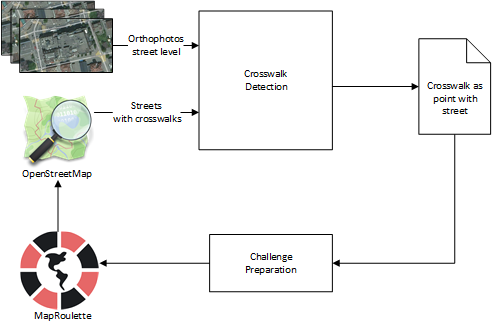
\includegraphics[width=\textwidth]{images/management_summary_1.png}
\caption[Überblick]{Überblick}
\end{figure}
\section*{Ausblick}
Das Projekt bietet viele Ausbaumöglichkeiten und kann nich nur auf Zebrastreifen angewendet werden. Es ist auch Denkbar auf den Strassen nach Markierungen zu suchen, wie Stop oder Bus etc.